%-*-coding: utf-8-*-

\chapter{Описание предложенного решения}

В данной главе будут рассмотрены предложенные идеи архитектур нейронных сетей на основе дерева разбора предложения.

В разделе \ref{ideas} будут кратко описаны предложенные идеи и мотивация их использования.

В разделе \ref{formal} будет дано формальное описание модели.

\section{Предложенные идеи} \label{ideas}

\subsection{Контекст слов в предложении}

Минусом подхода РТНС является то обстоятельство, что для поддеревьев с небольшим количеством слов (до 4-5 слов), методу сложно построить векторное представление достаточно точно, ввиду отсутствия контекста использования слов.\\
Так, в данном примере классификации эмоционального тона:

\begin{figure}[h]
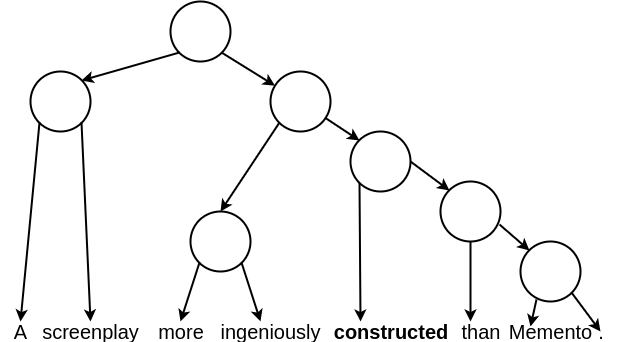
\includegraphics[scale=0.6]{Context_Example2}
\caption{\textbf{Пример зависимости от контекста}}
\label{fig:context_ex}
\end{figure}
Слово {\fontfamily{cmss}\selectfont \textbf{constructed}} не несет смысловой нагрузки для задачи, и поэтому для него сложно построить точное векторное представление относительно решаемой задачи.

Однако в контексте слов {\fontfamily{cmss}\selectfont \textbf{than Memento}} становится понятно, что это сравнительная фраза, и построить векторное представление в контексте задачи становится проще.

Данная проблема наталкивает на мысль: учитывать слова, 
использующиеся вместе с каждым словом в предложении, перед передачей в РНТС.

\subsection{Значимые слова в предложении}
Еще одной проблемой существующих решений, является то,  что они учитывают все слова предложения, 
хотя достаточно большое количество слов не несет смысловой нагрузки для решаемой задачи, а также для построения взаимосвязей
между словами.
Это требует от модели более избирательного анализа слов, а также порождает проблему \textquote{затухания градиента}, из-за 
длинной последовательности вычислений.

Рассмотрим следующий примеры для задачи классификации эмоционального тона предложения на датасете, состоящем из
обзоров кинофильмов.

{\fontfamily{cmss}\selectfont A \textbf{screenplay more ingeniosly} constructed \textbf{than Memento}.}

{\fontfamily{cmss}\selectfont Suffers from the \textbf{lack} of a \textbf{compelling} or \textbf{comprehensible narrative}.}

{\fontfamily{cmss}\selectfont Still, this \textbf{flick is fun} and \textbf{host to} some truly \textbf{excellent sequences}.}

\noindent Жирным выделены слова, которе несут основную смысловую нагрузку предложения.\\
Можно видеть, что достаточно большой процент от общего количества слов в предложении составляют 
\textquote{незначимые} для задачи слова.

Данная идея как раз и состоит в выделении наиболее значимых слов и фраз в предложении.
Эту идею можно обобщить на дерево разбора.

\section{Формальное описание алгоритма} \label{formal}

\subsection{Предобработка данных} \label{prework}
Для того чтобы алгоритм смог проанализировать предложение, 
его необходимо привести к определенному формату. Мы рассмотрим обработку
тренировочных данных, обработка тестовых данных производится аналогично.

В первую очередь, предложение необходимо разбить на слова. 
Это можно сделать используя регулярные выражения. 

Затем по данному корпусу предложений необходимо построить словарь слов.
Словарь~--- это некоторое подмножество слов предложений корпуса.
Это делается для того, чтобы ограничить объем вычислений, так как использование всех
слов языка достаточно ресурсоемко. Обычно в словарь попадают слова, 
имеющие наибольшую частоту использования в данном корпусе, 
либо просто все слова корпуса.

Те слова из корпуса, которые не попали в словарь заменяются специальным словом $UNK$, 
оно также добавляется в словарь.

Теперь необходимо для предложения построить дерево синтаксического разбора.
В рамках данной работы мы будем делать это, используя готовое решение $Stanford$ [ссылка].

При тестировании модели, производится аналогичная предобработка, 
с тем лишь отличием, что используется словарь, построенный по тренировочным данным.

Заметим, что весь процесс предобработки предложений автоматизирован, 
и не требует вмешательства человека.

\subsection{Построение векторного представления слов} \label{word_embedding}
После того, как построен словарь, каждому слову $w$ из словаря сопоставляется целочисленный индекс $i_w$ 
от $0$ до $N-1$, где $N$~--- размер словаря.
Каждое слово в словаре задается вектором размерности $N$, 
в котором на позиции $i_w$ находится единица, а на остальных позиция~--- нули.

Оперированием данным вектором напрямую в вычислениях~--- ресурсоемко, поэтому вводится вещественная матрица $W$, размерности $N \times d$, где $N >> d$.\\
Тогда вектор для слова $w$ вычисляется как
$$a_w = E_{i_w} \cdot W$$
где $E$~--- единичная матрица $N \times N$.\\
Таким образом мы построили векторное представление для слов из словаря, которое задается матрицей $W$.

Матрица $W$ является обучаемым параметром, и инициализируется либо произвольными числами, 
либо же используются предобученные на больших корпусах данных векторные представления, 
такие как word2vec или GLoVe [ссылки].

\subsection{Описание идеи \textquote{локальный контекст слов}} \label{loc_context}

Формально, предложение задается матрицей в  $\mathbb{R}^{l \times{} d}$, в которой $i$-я строка равна векторному представлению слова на позиции $i$,\\
где $l$~--- количество слов в предложении,\\
$d$~--- размерность векторного представления слов. 

Наша задача: получить новую матрицу в $\mathbb{R}^{l \times {} t}$, где $i$-я строка задает векторное представление \textit{контекста} данного слова в предложении. 
Данная операция задается оператором $F:\mathbb{R}^{l \times d} \to \mathbb{R}^{l \times t}$.

В рамках данной работы мы рассмотрим такие операторы $F$, которые в качестве контекста
для слова $i$ используют $k$-грамму с началом в $i$.\\
$k$-грамма~--- это слова на таких позициях $j$, что $i \le j < i + k$, где $k \in \mathbb{N}$~--- фиксированное значение и является параметром алгоритма.\\
Оператор $F$ такого вида определяется оператором
$C:\mathbb{R}^{k \times d} \to \mathbb{R}^t$, который определяет способ 
получить векторное представление из смежных слов. \\
Тогда $$F(X)_i = C(X'_{i..i+k-1})$$
где $X'$~--- это $X$ c добавленными в конец $k-1$ строками из нулей, \\
$X'_{i..i+k-1}$~--- матрица, образованная строками $X'$ c $i$ по $i+k-1$.\par

\vspace{5mm}

\noindent В данной работе будут использоваться следующие операторы $C$:
\begin{itemize}
    \item{полносвязный слой}
        $$C_{FC}(X)=\sigma(X^T \cdot W + b)$$
        где $W \in R^k, b \in R^d$, в данном случае $t=d$
    \item{сверточная нейронная сеть}
        $$c_j(X)=\sigma(X \odot m_j + b_j)$$
        $$C_{CNN}(X)=[c_1(X); c_2(X); \cdots c_t(X)]$$
        где $m_j \in \mathbb{R}^{k \times d}, b_j \in \mathbb{R}$,\\
        $\odot$~--- поэлементное произведение и суммирование полученных произведений, 
        так называемая операция \textquote{свертки}
    \item{долгая краткосрочная память}
    $$h_i=LSTM_h(c_{i-1},h_{i-1}, X_i) \text{ для } i \text{ от } 1 \text { до } k$$  
    $$c_i=LSTM_c(c_{i-1}, h_{i-1}, X_i) \text{ для } i \text{ от } 1 \text { до } k$$ 
    $$c_0 = \emptyset, h_0 = \emptyset$$
    $$C_{LSTM}(X) = h_k$$
    где $LSTM$~--- ячейка долгой краткосрочной памяти, описанной в разделе \ref{lstm} \\
    $LSTM_h, LSTM_c$~--- вычисление векторов $c$ и $h$ из $LSTM$ ячейки соответственно,\\
    $h_i \in \mathbb{R}^t, c_i \in \mathbb{R}^t$
\end{itemize}

\noindent Эта идея была названа \textquote{локальный контекст слов}.

\subsection{Описание идеи \textquote{значимые поддеревья}} \label{mean_subtree}

Перед нами стоит задача: вычислить для каждой вершины дерева разбора 
векторное представление фразы, соотвествующей этой вершине.
Мы будем делать это восходящим образом, вычисляя векторное представление для листьев,
затем для их предков, и так далее до корня дерева.

Обозначим векторное представление вершины $v$ за $f_v \in \mathbb{R}^s$.
Для вычисления $f_v$ в поддереве вершины $v$ будем выбирать такие поддеревья, 
что соответствующие им фразы являются наиболее значимыми для решаемой задачи.

Введем для каждой вершины $u$ весовой вектор $w_u \in \mathbb{R}^p$  так, что
чем больше квадрат нормы  этого вектора, тем более значима фраза, соотвествующая $u$.

Теперь чтобы посчитать векторное представление вершины $v$, выберем $K(v)$ вершин
в ее поддереве с наибольшими значениями $\lVert w_u \rVert^2$, пусть это $\{ u'_1, u'_2, \dots u'_{K(v)} \}$.
Затем с помощью некоторого оператора $G_v:\mathbb{R}^{K(v) \times s} \to \mathbb{R}^s$, 
передав в него выбранные значения $f_{u'_i}$, посчитаем векторное представление $f_v$.
Теперь остается пересчитать $w_v$. Сделаем это аналогичным образом, используя некоторый оператор 
$W_v :\mathbb{R}^{K(v) \times (s + p)} \to \mathbb{R}^p$, $f_{u'_i}$ и $w_{u'_i}$.

Формально:
$$TopK_v \{ \lVert w_{u_1} \rVert^2, \lVert w_{u_2} \rVert^2, \dots, \lVert w_{u_{2n-1}} \rVert^2\} = \{u'_1, u'_2, \dots, u'_{K(v)}\}$$
$$f_v = G_v(f_{u'_1}, f_{u'_2}, \dots, f_{u'_{K(v)}})$$
$$w_v = W_v(f_{u'_1} \circ w_{u'_1},f_{u'_2} \circ w_{u'_2}, \dots, f_{u'_{K(v)}} \circ w_{u'_{K(v)}})$$

\noindent $n$~--- количество слов в фразе, соответствующей вершине $v$\\
$u_1, u_2, \dots u_{2n-1}$~--- вершины поддерева $v$ в порядке эйлерова обхода\\
$TopK_v$~--- функция, которая выбирает $K(v)$ наибольших значений и возвращает их порядковые номера\\
$K(v)$~--- функция, которая определяет количество значимых поддеревьев для вершины $v$\\
$\circ$~--- операция конкатенации двух векторов в один

Мы можем видеть, что данный подход задается семействами операторов $G_v$ и $W_v$, и функцией $K$.

Также заметим, что если у нас уже есть вектора $f_v$, посчитанные некоторой другой моделью, не зависящей от данного подхода,
мы можем с помощью данного метода посчитать еще одни вектора $f'_v$ используя $f_v$, просто заменив во второй формуле $f_v$ на $f'_v$. И для предсказания использовать пару $(f_v, f'_v)$. Здесь нам по сути важен только $f'_{root}$, так как $f'_v$ не участвует в рекурсивных вычислениях.

Эта идея была названа \textquote{значимые поддеревья}.

\subsection{Архитектура и обучение модели} \label{arch}

Архитектуру полученной модели можно условно разбить на три части
\begin{enumerate}
    \item{подсчет векторного представления локального контекста}
    \item{подсчет векторного представления поддеревьев}
    \item{способ решения поставленной задачи по векторному представлению корня}
\end{enumerate}

Первый пункт был формально описан в разделе \ref{loc_context}

Раздел \ref{mean_subtree} описывает предложенный механизм для подсчета векторного представления поддеревьев.
Помимо предложенного решения, в рамках данной работы используется простая рекуррентная модель пересчета поддеревьев [статья], которая задается как:
$$f_v = \sigma(f_l \cdot W_1 + f_r \cdot W_2 + b)$$
где $f_v$~--- векторное представление вершины $v$, а $f_l$ и $f_r$~--- непосредственных
потомков веришы $v$,\\
$W_1, W_2 \in \mathbb{R}^{s \times s}$,
$b \in \mathbb{R}^s$~--- параметры рекуррентной модели

А также, древовидная LSTM модель [статья], которая задается как:
$$\tilde{i}_v=\sigma \left( U_1^{(i)} \cdot h_{v,1} + U_2^{(i)} \cdot h_{v,2} + b^{(i)} \right)$$
$$\tilde{f}_{vk}=\sigma \left( U_1^{(f)} \cdot h_{v,1} + U_2^{(f)} \cdot h_{v,2} + b^{(f)} \right),\text{ }k=1,2$$
$$\tilde{o}_{v}=\sigma \left( U_1^{(o)} \cdot h_{v,1} + U_2^{(o)} \cdot h_{v,2} + b^{(o)} \right)$$
$$\tilde{u}_{v}=\tanh \left( U_1^{(u)} \cdot h_{v,1} + U_2^{(u)} \cdot h_{v,2} + b^{(u)} \right)$$
$$\tilde{c}_v=\tilde{i}_v \odot \tilde{u}_v + \tilde{f}_{v,1} \cdot \tilde{c}_{v, 1} + \tilde{f}_{v,2} \cdot \tilde{c}_{v, 2}$$
$$\tilde{h}_v=\tilde{o}_v \cdot \tanh(\tilde{c}_v)$$

Способ решения задачи по векторному представлению корня непосредственно зависит от самой задачи.
То есть для каждой, отдельно взятой задачи, строится модель $G$, которая задается набором параметров $S$.
Модель $G$ принимает на вход $f_{root}$ и возвращает значение из области значений решаемой задачи. 
Набор параметров $S$ тренируется вместе с параметрами предложенной модели. Построение $G$ выходит за рамки данной работы, так как зависит от задачи, но мы рассмотрим $G$ для задач, использующихся в данной работе.

В данной работе нам потребуется решать задачу классификации предложения.
Для нее будет использоваться полносвязный слой c последующей softmax-функцией активации. 
В качестве функции потери используется кросс-энтропийная функции ошибки.\\
Формально:
$$z=f_{root} \cdot W_{out} + b_{out}$$
$$\tilde{y}_j=\frac{e^{z_j}} {\sum_{k=1}^K e^{z_k}}, j=1..K$$
$$L_2 = -\sum_{i=1}^K y_i \cdot \log(\tilde{y_i})$$
где $f_{root} \in R^s$~--- векторное представление корня\\
$K$~--- количество классов в задаче классификации\\
$W_{out} \in \mathbb{R}^{s \times K}, b_{out} \in \mathbb{R}^K$~--- параметры полносвязного слоя\\
$y_j$~--- правильный ответ для данного входного примера\\
$\tilde{y}_j$~--- распределение вероятностей по классам задачи классификации, сгенерированное моделью\\
$L_2$~--- значение ошибки на данном входном примере.\\
Оптимизация модели состоит в минимизации суммы $L_2$ по всем тренировочным данным.

\subsection{Архитектурные решения}
В данной работе были протестированы различные архитектуры:

\textbf{C подсчетом локального контекста слов}\\
В данной архитектуре варировались операторы, вычисляющие локальный контекст окна, размер окна $k$ и функция, вычисляющая векторные представления поддеревьев.

\textbf{C пересчетом поддеревьев методом значимых поддеревьев}\\
В данной архитектуре варировались операторы, вычисляющие векторное представление поддерева по значимым поддеревьям.

\textbf{С обоими предложенными подходами}\\
В данной архитектуре варировались операторы, вычисляющие локальный контекст окна, размер окна $k$.

\vspace{5mm}
Также была протестирована архитектура, которая использует векторное представление предложенного алгоритма как вспомогательный вектор, передающийся в $LSTM$ для предложения, а выходной вектор $LSTM$ используется, как описано в конце раздела \ref{arch}.